\PassOptionsToPackage{unicode=true}{hyperref} % options for packages loaded elsewhere
\PassOptionsToPackage{hyphens}{url}
%
\documentclass[
  12pt,
  twoside,
  banjiao]{ctexbook}
\usepackage{lmodern}
\usepackage{amssymb,amsmath}
\usepackage{ifxetex,ifluatex}

\usepackage{unicode-math}
\defaultfontfeatures{Scale=MatchLowercase}
\defaultfontfeatures[\rmfamily]{Ligatures=TeX,Scale=1}

% use upquote if available, for straight quotes in verbatim environments
\IfFileExists{upquote.sty}{\usepackage{upquote}}{}
\IfFileExists{microtype.sty}{% use microtype if available
  \usepackage[]{microtype}
  \UseMicrotypeSet[protrusion]{basicmath} % disable protrusion for tt fonts
}{}

\usepackage{xcolor}
\usepackage{xurl} % add URL line breaks if available
\usepackage{bookmark}
\usepackage{hyperref}
\hypersetup{
  pdftitle={免疫学},
  pdfauthor={github},
  pdfborder={0 0 0},
  breaklinks=true,
  bookmarksdepth=4}
\urlstyle{same}  % don't use monospace font for urls
\usepackage{longtable,booktabs}
% Allow footnotes in longtable head/foot
\IfFileExists{footnotehyper.sty}{\usepackage{footnotehyper}}{\usepackage{footnote}}
\makesavenoteenv{longtable}
\usepackage{graphicx,grffile}

\setlength{\emergencystretch}{3em}  % prevent overfull lines
% Redefines (sub)paragraphs to behave more like sections
\ifx\paragraph\undefined\else
  \let\oldparagraph\paragraph
  \renewcommand{\paragraph}[1]{\oldparagraph{#1}\mbox{}}
\fi
\ifx\subparagraph\undefined\else
  \let\oldsubparagraph\subparagraph
  \renewcommand{\subparagraph}[1]{\oldsubparagraph{#1}\mbox{}}
\fi

% set default figure placement to htbp
\makeatletter
\def\fps@figure{htbp}
\makeatother

\usepackage{multirow}
\usepackage{ctex}
\usepackage{rotating}
\usepackage{tablefootnote}
\setCJKmainfont{思源宋体}
\setCJKfallbackfamilyfont{\CJKrmdefault}{宋体}
\setmainfont{思源宋体}
\usepackage[a4paper,top=1in, bottom=1in, left=0.8in, right=0.8in]{geometry}
\setlength{\parindent}{2em}
\setlength{\parskip}{0em}

%\newfontfamily\apostrophefont[Ligatures=TeX,Color=FF0000]{Liberation Serif}
\newfontfamily\apostrophefont[Ligatures=TeX]{Liberation Serif}
\XeTeXinterchartokenstate=1
\newXeTeXintercharclass \apostrophe

% Assign the new class to all Latin capital letters
\makeatletter
\@tempcnta=`'
\loop\unless\ifnum\@tempcnta>`'
  \XeTeXcharclass \@tempcnta \apostrophe
  \advance \@tempcnta by 1
\repeat
\makeatother

% Setup font change
\XeTeXinterchartoks 0 \apostrophe   = {\begingroup\apostrophefont}
\XeTeXinterchartoks \apostrophe 0   = {\endgroup}
\XeTeXinterchartoks 4095 \apostrophe = {\begingroup\apostrophefont}
\XeTeXinterchartoks \apostrophe 4095 = {\endgroup}

\renewcommand {\thetable} {\thechapter{}-\arabic{table}}
\renewcommand {\thefigure} {\thechapter{}-\arabic{figure}}

\title{免疫学}
\author{github \\ \url{https://github.com/scienceasdf/medical-books}}

\begin{document}
\maketitle

{
\setcounter{tocdepth}{1}
\tableofcontents
\addcontentsline{toc}{chapter}{目录}
}
\newpage

\chapter{住院病人的营养评价}

\hypertarget{text00002.htmlux5cux23mllj1}{%
\section{ 住院病人营养不良现状和营养筛查}\label{text00002.htmlux5cux23mllj1}}

\hypertarget{text00002.htmlux5cux23mllj2}{%
\subsection{住院病人营养不良现状}\label{text00002.htmlux5cux23mllj2}}

先从小儿来讲,营养不仅是维持机体内环境稳定的基本物质,也是儿童自身生长发育所需要的基本物质。如果儿童营养不良,其免疫系统和其他脏器功能易受机体内外因素影响,易发生感染,营养相关并发症和死亡率增高。婴幼儿早期营养不良,可以导致远期认知功能和行为发育落后。Renaudin研究发现重度营养不良的患儿死亡率明显增高,30%的患儿死亡与营养不良有关。数十年来随着社会进步和经济发展,儿童营养不良发生率有所下降,但超重和肥胖发生率上升成为美国等发达国家儿童的重要问题。美国1981年198例住院儿童中急性营养不良发病率为54%。Hendricks对波士顿一家医院住院儿童营养状况研究时发现,1992年急性和慢性营养不良发生率明显低于该院1976年水平。而Cynthia发现美国6~11岁儿童超重发生率从20世纪60年代的6%上升到80年代的11%,到20世纪末,甚至高达15.3%。但在发展中国家,儿科病人营养不良发生率仍然很高。1983年,40492例阿富汗住院患儿中,67%具有不同程度的营养不良。泰国1995年住院患儿营养不良的发生率和10年前相似,达到50%~60%。2003年巴基斯坦1878名<3岁的儿童中,患急、慢性营养不良者的比例分别为26%、55%,同时兼有急性和慢性营养不良的比例为15%。2000年发展中国家<5岁儿童低体重的发病率与1980年的37.4%相比有所下降,但仍高达26.7%。而患儿的营养状况往往被临床医生所忽视。2003年我们对上海3家儿童医院2274例住院儿童进行营养评价,发现生长迟缓(HAZ<-2)、消瘦(WAZ-2)、低体重(WAZ<-2)发生率分别为20.6%、21.5%、22.2%,表明营养不良发生水平较高。因此,有必要对所有儿科住院病人进行营养评价。

据国内研究显示,住院病人营养不良的发生率为15%~60%,其中约50%属于严重营养不良。营养不良可能导致并发症发生率上升、住院时间延长、疾病恢复缓慢、医疗费用增加,而进行营养评价并进行合理的营养支持有利于改善上述情况。据最新研究报道,在家庭居住的老年人营养不良发生率占5%~10%,住院或在老年院居住者高达30%~60%,由于各种急、慢性疾病短期或长期影响,营养不良在老年人中有较高的发生率。北京协和医院于康等的调查显示,外科老年住院病人营养不良高达41.6%,有发生营养不良危险者占20.8%,两者都高于中青年病人。有资料分析,住院病人死亡病例中的1/3死因并非是疾病本身,而是营养不良所致。如果病人在1个月内体重急剧减轻达20%以上,不管其发病原因是什么,都会因营养衰竭而死亡。经临床确认,住院病人的蛋白质热量营养不良的发生率高达40%~60%。因此,营养治疗与药物、手术、护理及其他专门疗法具有同等重要性,给病人住院提供足够的营养,可以增强机体抵抗力,减少并发症,促进伤口愈合,防止营养不良的发生。

\hypertarget{text00002.htmlux5cux23mllj3}{%
\subsection{营养状况筛查}\label{text00002.htmlux5cux23mllj3}}

营养状况筛查应该简单且快速,否则繁忙的医护人员难以有效地进行筛查。营养筛查还应该具有足够的敏感度,能够检测到几乎所有病人营养缺乏的危险性。在检查营养状况的同时需考虑病人所患其他疾病的严重性,有助于进行正确的判断,因为这两者经常互相作用,如中度营养不良伴有严重疾病时,两者相互影响就会比较明显。筛查的结果应该以能量化且可以审核的指标表示,之后应该进行合适和准确的处理。

大多数营养筛查会筛查4个方面的问题:近期体重的变化;近期膳食摄入状况;近期体质指数以及近期疾病的状况或其他导致营养不良的危险因素。在2003年,欧洲肠外与肠内营养学会(ESPEN)制定了社区、医院及老年人群营养状况筛查的原则,即预测性、稳定性和实用性。对于成年住院病人的营养筛查推荐使用“2002营养不良危险因素筛查表”,即进行第一步预筛查(表1-1)。如果根据这个筛查表得分≥3则病人需要制定营养改善计划,如果病人存在营养不良的风险,但同时存在代谢或功能问题,无法实施一般的营养改善方案,或不确定病人是否存在营养不良风险时,就必须转诊请专家作进一步更为详细的营养评价,即进行第二步正式筛查(表1-2)

\begin{table}[htbp]
{\centering
\caption{第一步预筛查}
\label{tab1-1}

\includegraphics{./images/Image00000.jpg}}

注:以上如有1个问题的回答为“是”,则进行第二步筛查;如每个问题的回答都为“否”,病人在以后每周进行1次初步筛查。
\end{table}



\begin{table}[htbp]
{\centering
\caption{第二步正式筛查}
\label{tab1-2}

\includegraphics{./images/Image00001.jpg}}

{注:NRS 2002的制定依据现有的随机临床试验}

{*表明确诊的病人可直接归为此类。用黑体字标注的病例按照下面介绍的疾病严重程度标准进行归类:}

{营养不良危险因素是指机体目前的营养状况以及因此可能导致的机体损害,因为在病理状况下机体代谢压力加大,对营养素的需要量也有所增加。}

{营养干预对于下列病人是必需的:}

{1)严重的营养不良(3分);}

{2)严重疾病(3分);}

{3)中度营养不良+轻度疾病(2分+1分);}

{4)轻度营养不良+中度疾病(1分+2分)。}

{1分:病人患有慢性疾病并因并发症而住院,身体虚弱但可以定时下床活动。病人对蛋白质的需要量增加,但对于大多数病例通过正常膳食或口服营养素补充剂就可以满足需要。}

{2分:病人卧床休息,如胃部外科大手术。病人对蛋白质的需要量大大增加,一些病人必须通过人工喂养才能满足需要。}

{3分:重症监护病人,如使用呼吸机的病人。病人对蛋白质的需要量增加,并且通过人工喂养也不能满足需要。蛋白质分解和氮丢失显著减少。}
\end{table}



\hypertarget{text00002.htmlux5cux23mllj4}{%
\section{营养评价内容及方法}\label{text00002.htmlux5cux23mllj4}}

\hypertarget{text00002.htmlux5cux23mllj5}{%
\subsection{疾病及饮食史}\label{text00002.htmlux5cux23mllj5}}

疾病史包括急、慢性疾病回顾以及既往营养丢失情况。饮食史多采用24小时膳食回顾或3天连续食物称重法,应该同时考虑食物的数量和质量,将能量、蛋白质和微量营养素与推荐摄入量(DRIs)进行比较。Beck使用体重和食欲下降对入院病人进行初筛,然后通过主观全面评价法对营养不良疑似病人进一步评价,发现其中营养不良比例高达63%。膳食评价可以在病人入院早期发现营养问题,给予营养支持,改善病人预后。

\hypertarget{text00002.htmlux5cux23mllj6}{%
\subsection{体格测量}\label{text00002.htmlux5cux23mllj6}}

{1.体重}
 体重是临床上最常用的体格检查指标,但目前还没有完全做到记录每个住院病人的体重。短期体重变化是反映体液平衡的最佳指标。较长期的体重改变能够反映总体营养状况改变,根据病前3~6个月的体重变化或实际体重占理想体重的百分比,来判断是否需要进一步检查评估。3个月内非自愿的体重减轻是评价机体营养状况的有用指标,体重减轻<5%为轻度,体重减轻>10%为重度。如果病人体重持续减轻,临床医师应该对此警惕并找出原因。在儿科病人中,联合应用体重和身高,可以转换成多种指标对营养状况进行监测,如身高别体重(W/H)可以判断是否存在急性营养不良及其程度,年龄别身高(H/A)用来判断是否存在慢性营养不良及其程度。身高别体重比年龄别体重更能反映近期或进行性体重丢失,与预后相关,而年龄别体重(W/A)低下并不会导致患儿死亡率的明显升高。

体质指数(BMI)是目前临床上常用的另一项体重/身高关系指数,等于体重与身高平方的比值,多用于成人或肥胖儿童营养评价。亚洲人的BMI
18.5~24为正常,>24为超重,<18.5为营养不良,<14为严重营养不良,这种病人存活的可能性很小。个体BMI不仅要与以上标准进行比较,而且还要与本人近期的数值进行比较,这样意义会更大。Tienboon将BMI应用于身高<145cm的儿童,如BMI在13.0~14.5代表轻度营养不良,11.5~12.9为中度营养不良,<11.5为重度营养不良。

{2.皮褶厚度测量}
 可用来估计体脂含量,因为总体脂肪和某些特定部位的皮褶厚度之间存在一定的比例关系,通常选择测量上臂肱三头肌皮褶厚度(TSF),其次是选择肩胛下角处皮褶厚度。慢性营养不良的病人常见有皮褶厚度的减低。由于重症病人TSF受总体脂肪变化的影响,而且不同人群由于年龄、性别及疾病的不同,皮下脂肪与总体脂肪的比值可以在0.2~0.7之间变动,测量精确性差,往往高估消瘦病人的体脂含量,而低估肥胖者的体脂含量。不同部位皮褶厚度测量值之和可以更为准确反映病人体脂含量。

{3.中臂围(MAC)}
 是用卷尺测量肩峰和尺骨鹰嘴中点的手臂围,这个指标易测量且误差也较小。中臂围与某些疾病的死亡率、发病率等指标有很好的相关性,它主要是测量身体的总成分,包括肌肉、骨骼、体液和脂肪组织等,当蛋白质及脂肪储备下降时MAC迅速减少。根据TSF和MAC可以计算中臂肌围、臂脂肪面积、臂肌面积,用于反映脂肪和瘦体组织含量。

{4.头围(HC)}
 HC是3岁以内儿童生长发育和营养状况评价的常用指标,可以间接反映大脑发育情况,如婴儿期头围增长缓慢,将来出现发育问题的风险明显增高。中臂围与头围比值(MAC/HC)受体液变化的影响较小,是新生儿、婴儿营养评价及监测中筛选营养不良的敏感指标。

\hypertarget{text00002.htmlux5cux23mllj7}{%
\subsection{生化指标}\label{text00002.htmlux5cux23mllj7}}

(一)蛋白质营养状况

{1.白蛋白}
 白蛋白的代谢半衰期是18天,所以其代谢变化对浓度的影响需要一段时间才能显现出来。白蛋白从血液中正常流失的速度是其合成速度的10倍。营养不良的病人,机体内脏蛋白储备丧失,血浆蛋白尤其是快速转化蛋白多有降低。血浆白蛋白是评价营养状况的常用指标,白蛋白浓度明显降低常常导致感染发生率和死亡率增高。

{2.前白蛋白和转铁蛋白}
 前白蛋白和转铁蛋白半衰期短,前者为2天,后者为7天,它们对营养状况变化敏感,是判别蛋白质营养不良的良好指标。实验证明,血清前白蛋白浓度在肠外营养应用1周后明显升高(P<0.001),而应用白蛋白则无改变。Staffan对28位极低体重出生儿进行11种血浆蛋白质测定,发现前白蛋白、转铁蛋白、视黄醇结合蛋白最适合该人群蛋白质营养状况评价。

{3.纤维连接蛋白}
 纤维连接蛋白在饥饿状态下迅速降低,给予营养补充后很快恢复正常,因此也可以作为营养评价的指标。

{4.血红蛋白}
 营养性贫血是最常见的营养问题,美国第三次营养与健康调查发现1~3岁儿童缺铁性贫血发生率为15%。上海新华医院对上海3家儿科医院进行调查,贫血发生率为29.3%。血红蛋白和血细胞比容测定可以诊断营养性缺铁性贫血,转铁蛋白浓度与总体铁储备密切相关,是正常人体铁状况的敏感指标。为病人进行血常规检查,对营养状况评价很有意义。

{5.肌酐}
 肌酐主要由肌氨酸代谢分解产生,因此尿肌酐清除率可作为估计瘦体组织的可靠指标。肌酐身高指数(CHI)常用来估计肌肉蛋白质储备,CHI在60%~80%为中度蛋白质缺乏,<60%为重度蛋白质缺乏。

{6.其他}
 3-甲基组氨酸测定结果也可以反映肌肉蛋白储备和运转情况,但它和肌酐清除率都存在一定问题,如难以准确收集24小时尿量,受饮食和肾功能影响很大,尚不推荐常规应用。肝脏中酶的活性以及电解质水平(钙、磷、镁等)都应常规检测。锌、硒和铁的检测对于胃肠道病人尤其重要。

(二)免疫功能测定

慢性阻塞性肺病(COPD)病人的营养状况与其细胞免疫功能密切相关,一般把免疫功能的评价作为营养状况评价的重要组成部分。

{1.外周血总淋巴细胞计数}
 外周血总淋巴细胞计数(TLC)指外周血中总淋巴细胞的数量,可反映细胞免疫功能。TLC=白细胞×淋巴细胞百分比,正常值≥1.5×10\textsuperscript{9}
/L,营养不良时TLC下降。

{2.迟发型超敏皮肤试验}
 于前臂屈侧皮内注射不同的抗原制剂0.1ml,待48小时测量接种处硬结直径。常用的抗原包括链激酶、腮腺炎病毒、白色念珠菌提取液、植物血凝素、结核菌素纯蛋白衍生物等。营养不良时细胞免疫功能受损,迟发型超敏皮肤试验为无反应或反应减弱,即接种处不出现硬结或硬结直径很小。

{3.外周血T细胞亚群}
 机体T细胞的免疫应答反应对抵抗力或免疫功能非常重要,其中目前临床上常用的指标主要是$\text{CD}^+_3$
、$\text{CD}^+_4$
、$\text{CD}^+_8$
、$\text{CD}^+_4$
/$\text{CD}^+_8$ 等,营养不良时下降。

\hypertarget{text00002.htmlux5cux23mllj8}{%
\subsection{机体组成测定}\label{text00002.htmlux5cux23mllj8}}

构成机体的基本化学成分是蛋白质、脂质、碳水化合物、无机盐和水等。由于中性脂肪并不结合水和电解质,假设人体去脂体质(fat-free
mass, FFM)或瘦体群(lean body mass,
LBM)的组成是恒定的,那么通过分析其中一种组成(如水、钾或钠)的量可估计FFM的多少,然后用体重减去FFM的重量即为体脂(body
fat,
BF)。因此,机体的组成按照二元件模型可分为BF和FFM两部分。FFM可再分为体细胞群(body
cell mass, BCM)和细胞外群(extracellular mass,
ECM)。BF是机体储备能量的主要组织,约占体重的25%,其主要成分是脂肪。脂肪中仅有1.0kg脂肪为生命活动所必需,其余可在需要时被动员用于能量消耗。BCM是能够利用氧进行代谢活动的组织,约占人体总重量的40%。ECM主要是细胞外支持组织,用于支持细胞的功能和活动,约占人体重量的35%。在人体组成分析中,显然FFM较BF在生命活动和机体代谢方面更具有重要作用。测定人体组成及其变化比单纯体重指数更能客观反映病人实际的营养状况。

早在1940年,水中称重法应用于人体机体组成测定,来推算体脂和去脂体质的重量。空气置换体积描记术是一项新的密度测定方法,尤其适合那些无法耐受水中密度测定的儿童等特殊病人,David等在9~14岁儿童中应用发现该法比水中称重等方法能更精确测定体脂含量。因为水与钾仅存在于瘦体组织,且含量相对恒定,脂肪不含水和钾。因此通过放射性核素稀释法总体水测定和总体钾测定都可以计算总体脂肪和廋体组织含量。双能X线吸收法是测定人体骨骼无机盐、体脂、去脂组织等机体组成的常用方法,与总体钾测定相关性较好。但多用于研究机构,较少应用于临床评价。迟发性中子激活分析法能够测定氮、钠、氯、钾、钙、磷等多种原子的绝对水平,如测定总体氮可用于机体蛋白质组成分析。CT及磁共振能获得体脂分布的精确图像。

许多机体组成测定方法由于存在一些缺点,如费用昂贵、放射暴露、需要专门的测量仪器和场所,或是需要检查对象合作,而难以在临床上推广引用。生物电阻抗法(BIA)是近年来广泛用于机体组成测定的新方法,具有可床边进行,操作简便、快捷、安全、无创等优点。它的原理是利用不同生物组织对电流导电的差异性,低频电流主要通过细胞外液传导,高频电流可以穿透细胞膜,同时通过细胞内液和细胞外液,推测组织各部分的含量。基于此特性可推测总体水、瘦体组织、细胞外液和细胞团块等多种机体组成成分。Phillips使用BIA和放射性核素稀释法两种方法对青春期女性进行测定,认为BIA法能精确反映她们月经前和月经后去脂组织和体脂含量变化。

\hypertarget{text00002.htmlux5cux23mllj9}{%
\subsection{营养平衡研究}\label{text00002.htmlux5cux23mllj9}}

营养平衡研究一直用于营养评估,通过计算出入量,可进行氮、无机盐、维生素、微量元素等多种物质的平衡研究。氮平衡测定是一项重要的营养平衡研究方法,可直接判断蛋白质摄入情况,常用于营养治疗过程中观察病人的营养摄入是否足够以及了解分解代谢的演变。氮平衡首先测量人体通过尿液、粪便、皮肤以及其他途径(汗液、分泌液等)流失的氮,将摄入氮减去以上各种途径排出的氮就可以计算出氮平衡。为了确定蛋白质的需要量,氮平衡测定需在蛋白质从缺乏到过剩几种不同的摄入水平下进行。每个摄入水平的测定都需要持续几天,使机体保持代谢稳定。由于技术上的原因,目前按照以上要求进行的代谢试验较少,仍缺乏可用于临床病人的标准化方法。正氮平衡常常意味着预后改善,病人营养支持的目的是达到正氮平衡。但氮平衡不能反映机体的蛋白质储备或营养状态,需结合机体组成等测定综合评价。

\hypertarget{text00002.htmlux5cux23mllj10}{%
\subsection{复合型营养评定方法}\label{text00002.htmlux5cux23mllj10}}

{1.主观全面营养评估法(SGA)}
 SGA是Detsky在1987年首先提出,是根据病史和体格检查的一种主观评估方法,特点是以详细的病史与临床检查为基础,省略人体测量和生化检查。其理论基础是:身体组成改变与进食改变、消化吸收功能的改变、肌肉的消耗、身体功能及活动能力的改变等相关联。在重度营养不良时,SGA与身体组成评定方法有较好的相关性。此方法简便易行,适于在基层医院推广(表1-3)。

\begin{table}[htbp]
\centering
\caption{营养状态的SGA(subjective global assessment)评估内容和指标}
\label{tab1-3}
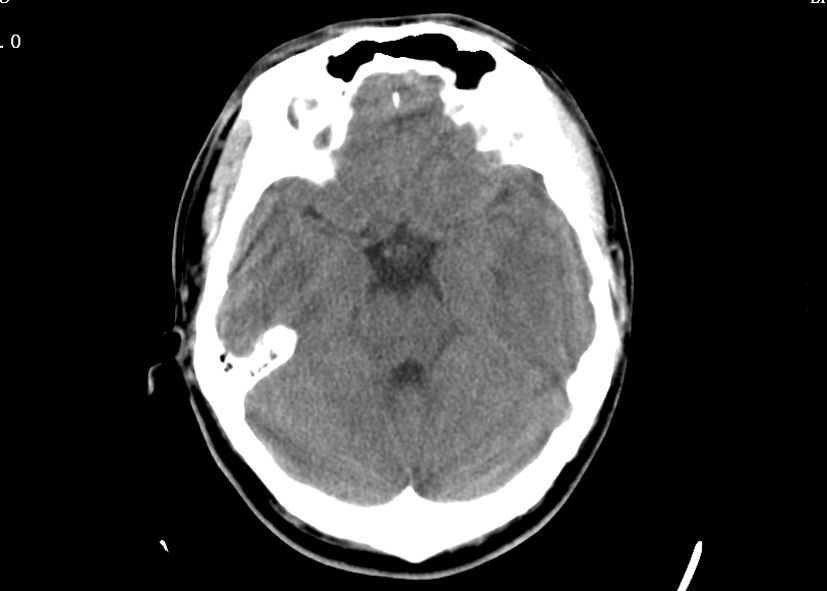
\includegraphics{./images/Image00005.jpg}
\end{table}

{2.预后营养指数(PNI)}
 PNI是由Mullen等对4种营养状态评价参数与外科手术病人预后的相关性进行了分析统计之后提出来的一种综合性营养评价方法。

PNI(%)=158-16.6(ALB)-0.78(TSF)-0.20(TFN)-5.80(DHST)

式中ALB为血清白蛋白(单位:g%);TSF为三头肌皮褶厚度(单位:mm);TFN为血清转铁蛋白(单位:mg%);DHST为迟发性超敏皮肤反应试验(硬结直径>5mm者,DHST=2;硬结直径<5mm者,DHST=1;无硬结反应者,DHST=0)。

评定标准:若PNI<30%,表示发生术后并发症及死亡的可能性均很小;若30%≤PNI<40%,表示存在轻度手术危险性;若40%≤PNI<50%,表示存在中度手术危险性;若PNI≥50%,表示发生术后并发症及死亡的可能性均较大。

Mullen等对161例非急诊手术病人的PNI测定调查显示,手术危险增加与术后并发症发生率及死亡率升高相关,其灵敏度为86%,特异性为69%。

{3.微型营养评定(MNA)}
 是一种简单、快速,适用于评价病人(特别是老年人)营养状况的方法,由Guigoz、Vallas和Garry于1994年提出。MNA评价内容包括: ①人体测量;②整体评定;③膳食问卷;④主观评定等。各项评分相加即得MNA总分。具体评价问卷内容如下所列(见[附])。

\begin{center}\rule{0.5\linewidth}{\linethickness}\end{center}

[附]

营养评价问卷

(一)姓名 性别 出生 年 月 日

(二)家庭住址

(三)原有疾病

(四)体重(kg) 身高(m) 血压(mm Hg)

1.筛选(按不同程度给予量化评分)

(1)既往3个月内是否有食欲下降、消化问题、咀嚼或吞咽困难而摄食减少?

0=食欲完全丧失□ 1=食欲中等度下降□ 2=食欲正常□

(2)既往3个月内体重下降

0=>3kg□ 1=不知道□ 2=1~3kg□ 3=无体重下降□

(3)活动能力

0=需卧床或长期坐着□ 1=能不依赖床或椅子,但不能外出□ 2=能独立外出□

(4)既往3个月内有无重大心理变化或急性疾病?

0=有□ 1=无□

(5)神经心理问题

0=严重智力减退或抑郁□ 1=轻度智力减退□ 2=无问题□

(6)BMI(kg/m\textsubscript{2} )

0=<19□ 1=19~<21□ 2=21~<23□ 3=≥23□

筛选总分(14):≥12正常,无需以下评价;≤11可能营养不良,继续以下评价

2.评价

(1)独立生活(无护理或不住院)?

0=否□ 1=是□

(2)每天应用处方药3种?

0=是□ 1=否□

(3)压疮(褥疮)或皮肤溃疡?

0=是□ 1=否□

(4)每天几次吃完全部饭菜?

0=1餐□ 1=2餐□ 2=3餐□

(5)蛋白质摄入情况:

*每天至少一份奶制品? A是□ B否□

*每周2份以上菜果或蛋? A是□ B否□

*每天肉、鱼或家禽? A是□ B否□

0.0=0或1个“是”□

0.5=2个“是”□

1.0=3个“是”□

(6)每天2份以上水果或蔬菜?

0=否□ 1=是□

(7)每天饮水量(水、果汁、咖啡、茶、奶等):

0.0=<3杯□ 0.5=3~5杯□ 1.0=>5杯□

(8)喂养方式:

0=无法独立进食□ 1=独立进食稍有困难□ 2=完全独立进食□

(9)自我评定营养状况:

0=营养不良□ 1=不能确定□ 2=营养良好□

(10)与同龄人相比,你如何评价自己的健康状况?

0.0=不太好□ 0.5=不知道□ 1.0=好□ 2.0=很好□

(11)中臂肌围(cm):

0.0=<21□ 0.5=21~22□ 1.0=≥22□

(12)腓肠肌围(cm):

0=<31□ 1=≥31□

评价总分(16):

筛选总分:

总分(30):

MNA分级标准:上述各项评分相加,若MNA≥24,表示营养状况良好;若17≤MNA≤23.5,表示存在发生营养不良的危险;若MNA<17,表示有确定的营养不良。

\begin{center}\rule{0.5\linewidth}{\linethickness}\end{center}

{4.住院病人预后指数(HPI)}

HPI=0.92(ALB)-1.00(DH)-1.44(SEP)+0.98(DX)-1.09

式中:ALB为血清白蛋白(单位:g/L);DH为延迟超敏皮肤试验(有1种或多种阳性反应,DH=1;所有均呈阳性,DH=2);SEP:败血症(有败血症,SEP=1;无败血症,SEP=2);DX表示诊断患有癌症(有癌,DX=1;无癌,DX=2)。

评价标准:若HPI为+1,表示有75%的生存概率;若HPI为0,表示有50%的生存概率;若HPI为-2,表示仅有10%的生存概率。

{5.营养风险指数(NRI)}
 美国退伍军人协会肠外营养协作研究组(VATPNCSG)于1991年在《新英格兰医学杂志》上首先提出NRI评价方法。NRI=10.7(ALB)+0.0039(TLC)+0.11(Zn)-0.044(Age)。

式中:ALB为血清白蛋白;TLC为淋巴细胞计数;Zn为血清锌水平;Age为年龄。

评定标准:若NRI>60,表示危险性低;若NRI≤55,表示存在高危险性。

Clugston等于2006年对梗阻性黄疸病人的研究表明,NRI风险升高与住院时间延长和死亡率增加相关。

完整的营养评价包括:疾病及饮食史、体格测量、生化指标、机体组成、营养平衡研究等。在营养评价过程中,体格测量与生化指标是营养评价的最常用方法,具有简单、方便、重复性好、能提供定量资料、不需要特殊仪器等特点。很多测量值与机体组成营养状况分析在统计学上具有显著相关性。然而,简单的体格测量和实验室检查常不能体现营养状况的急性改变,不能反映轻度和中度营养不良,也就不足以作为营养评价的唯一方法。同时,由于置信限较宽,敏感性和特异性差,更适用于流行病学人群调查,评价特定人群的营养状态。近年来,为了提高营养评价方法的敏感性和特异性,人们结合预后和大量的营养学指标,通过多因素回归分析,选择其中有意义的参数,组成最佳的预测模式,建立了多种营养评价方法,为营养状况评价提供了定性、定量的可信指标。

{参考文献}

[1]陶晔璇,徐远飞,汤庆娅,等.儿科病人入院时营养状况评价.中国临床营养杂志,2007,15(4):214~217

[2]蔡威.临床营养基础.第3版.上海:复旦大学出版社,2004,61~18

[3]Tienboon P. Nutrition problems of hospitalised children in a
developing country: Thailand. Asia Pacific J Clin Nutr, 2002, 11 (4):
258~262

[4]Renaudin P. Evaluation of the nutritional status of children less
than 5 years of age in Moundou, Chad: correlations with morbidity and
hospital mortality. Article in French. Med Trop(Mars), 1997, 57 (1):
49~54

[5]Hendricks KM, Duggan C, Gallagher L, et al. Malnutrition in
hospitalized pediatric patients. current prevalence. Arch Pediatr
Adolesc Med, 1995, 149: 1118~1122

[6]Ogden CL, Flegal KM, Carroll MD, et al. Prevalence and trends in
overweight among US children and adolescents, 1999~2000. JAMA, 2002,
288 (14): 1728~1732

[7]Ah SM, Selwyn BJ, Luby S, et al. Prevalence and correlates of
stunting among children in rural Pakistan. Pediatr Int, 2003, 45 (1):
49~53

[8]Jacobs DO, Wong M. Metabolic assessment. World J Surg, 2000, 24
(12): 1460~1467

[9]Phillips SM, Bandini LG, Compton DV, et al. A longitudinal
comparison of body composition by total body water and bioelectrical
impedance in adolescent girls. J Nutr, 2003, 133 (5): 1419~1425

[10]Kuczmarski RJ, Ogden CL, Guo SS, et al. 2000 CDC growth charts for
the United States: methods and development. Vital Health Stat 11, 2002,
(246): 1~190

[11]Ronald E. Pediatric nutrition handbook. 6th ed. American: American
Academy of Pediatrics, 2009, 559~576

\protect\hypertarget{text00003.html}{}{}



\end{document}
